% =============================================================================
%  BÁO CÁO ĐỒ ÁN OSG203 — LinuxAdmin Toolkit cho TechNova Solutions
%  Biên dịch bằng XeLaTeX (cần 2 lần để có mục lục):
%     xelatex bao-cao.tex && xelatex bao-cao.tex
%  hoặc không cần cài LaTeX:  ./build.sh   (dùng Docker image texlive/texlive)
%  >>> Sửa thông tin nhóm ở phần "THÔNG TIN NHÓM" ngay bên dưới <<<
% =============================================================================
\documentclass[12pt,a4paper,oneside]{report}

% ------------------------------------------------------------ THÔNG TIN NHÓM ---
\newcommand{\Truong}{TRƯỜNG ĐẠI HỌC .......................}
\newcommand{\Khoa}{KHOA CÔNG NGHỆ THÔNG TIN}
\newcommand{\MonHoc}{OSG203 — Hệ điều hành Linux}
\newcommand{\GiangVien}{.......................}
\newcommand{\Lop}{.......................}
\newcommand{\NhomSV}{%
  Nguyễn Văn A — MSSV ........ \\
  Trần Thị B — MSSV ........ \\
  Lê Văn C — MSSV ........}
\newcommand{\NgayNop}{TP. Hồ Chí Minh, tháng 10/2026}
\newcommand{\RepoURL}{https://github.com/duylmaoxd/technova-sysadmin-toolkit}

% ---------------------------------------------------------------- GÓI LỆNH ---
\usepackage{fontspec}
\usepackage{polyglossia}
\setdefaultlanguage{vietnamese}
\setmainfont{TeX Gyre Termes}
\setsansfont{TeX Gyre Heros}
\setmonofont{JetBrainsMono}[Path=fonts/, Extension=.ttf, UprightFont=*-Regular, BoldFont=*-Bold, Scale=0.82]
\usepackage[left=3cm,right=2cm,top=2.5cm,bottom=2.5cm]{geometry}
\usepackage{setspace}\setstretch{1.25}
\usepackage{graphicx,float,booktabs,tabularx,longtable,array,enumitem,caption,fancyhdr,xcolor,fancyvrb,colortbl}
\usepackage{tikz}\usetikzlibrary{positioning,arrows.meta,shapes.geometric,fit}
\usepackage[hidelinks,unicode]{hyperref}
\graphicspath{{../hinh/}}

\definecolor{navy}{HTML}{14324F}
\definecolor{teal}{HTML}{0F7C80}
\definecolor{mint}{HTML}{E6F4F1}
\definecolor{code}{HTML}{F4F6F8}
\definecolor{amber}{HTML}{E8A33D}

\setlist{itemsep=2pt,topsep=4pt}
\captionsetup{font=small,labelfont={bf,color=navy}}
\renewcommand{\arraystretch}{1.25}
\newcolumntype{L}{>{\raggedright\arraybackslash}X}

\fvset{fontsize=\small,frame=single,framesep=6pt,rulecolor=\color{teal!50},numbers=none}
\newcommand{\cmd}[1]{\texttt{\small #1}}

\pagestyle{fancy}\fancyhf{}
\fancyhead[L]{\small\color{navy}LinuxAdmin Toolkit — TechNova Solutions}
\fancyhead[R]{\small\color{navy}\MonHoc}
\fancyfoot[C]{\thepage}
\renewcommand{\headrulewidth}{0.4pt}

\makeatletter
\renewcommand{\@makechapterhead}[1]{%
  \vspace*{0pt}{\color{teal}\sffamily\large\bfseries \chapname\ \thechapter}\par\vspace{4pt}
  {\color{navy}\sffamily\huge\bfseries #1\par}\vspace{18pt}}
\renewcommand{\@makeschapterhead}[1]{%
  \vspace*{0pt}{\color{navy}\sffamily\huge\bfseries #1\par}\vspace{18pt}}
\makeatother
\renewcommand{\thesection}{\thechapter.\arabic{section}}
\newcommand{\chapname}{CHƯƠNG}

\begin{document}

% ---------------------------------------------------------------- TRANG BÌA ---
\begin{titlepage}
\begin{tikzpicture}[remember picture,overlay]
  \draw[navy,line width=2pt] ([xshift=2cm,yshift=-1.6cm]current page.north west) rectangle ([xshift=-1.6cm,yshift=1.6cm]current page.south east);
  \draw[teal,line width=0.6pt] ([xshift=2.2cm,yshift=-1.8cm]current page.north west) rectangle ([xshift=-1.8cm,yshift=1.8cm]current page.south east);
\end{tikzpicture}
\centering\sffamily
{\large\bfseries\color{navy}\Truong\par}
{\large\bfseries\color{navy}\Khoa\par}
\vspace{2.2cm}
{\Large\color{teal}BÁO CÁO ĐỒ ÁN MÔN HỌC\par}
{\large \MonHoc\par}
\vspace{1.4cm}
{\color{navy}\rule{0.6\textwidth}{1pt}\par}\vspace{0.4cm}
{\fontsize{24}{30}\selectfont\bfseries\color{navy}LINUXADMIN TOOLKIT\par}
\vspace{0.3cm}
{\Large\bfseries Bộ công cụ quản trị máy chủ bằng Bash\\cho doanh nghiệp TechNova Solutions\par}
\vspace{0.4cm}{\color{navy}\rule{0.6\textwidth}{1pt}\par}
\vspace{0.5cm}
{\large Đề tài 3: \textit{Bash Scripting cho System Administration}\par}
\vfill
\begin{tabular}{rl}
\textbf{Giảng viên hướng dẫn:} & \GiangVien \\[4pt]
\textbf{Lớp:} & \Lop \\[4pt]
\textbf{Sinh viên thực hiện:} & \begin{tabular}[t]{@{}l@{}}\NhomSV\end{tabular}
\end{tabular}
\vfill
{\NgayNop\par}
\end{titlepage}

% ---------------------------------------------------------------- TÓM TẮT ---
\chapter*{Tóm tắt}
\addcontentsline{toc}{chapter}{Tóm tắt}
Báo cáo trình bày quá trình phân tích, thiết kế, hiện thực và kiểm thử \textbf{LinuxAdmin Toolkit}. Đây là bộ công cụ quản trị máy chủ Linux viết hoàn toàn bằng Bash, phục vụ một kịch bản doanh nghiệp giả định: công ty \textbf{TechNova Solutions} có một máy chủ Ubuntu Server tập trung (\cmd{technova-core-srv}) cho toàn bộ lập trình viên, data analyst và tester SSH vào làm việc. Tech Lead của công ty làm việc từ xa và chỉ dùng terminal qua SSH để điều hành hệ thống.

Toolkit gom các công việc hằng ngày của Tech Lead vào \textbf{5 chức năng chính}:
\begin{enumerate}
  \item \textbf{users} — quản lý nhân viên và phân quyền;
  \item \textbf{monitor} — giám sát tài nguyên và hoạt động của nhân viên;
  \item \textbf{alert} — cảnh báo sự cố tức thời;
  \item \textbf{backup} — sao lưu tài sản số;
  \item \textbf{scheduler} — tự động hoá bảo dưỡng.
\end{enumerate}

Hệ thống có \textbf{hai chế độ làm việc} chuyển qua lại được: giao diện menu trong terminal (TUI, dùng \cmd{dialog}/\cmd{whiptail}) và dòng lệnh (CLI). Hai chế độ dùng chung một bộ chức năng, vì mỗi thao tác trên giao diện thực chất gọi đúng một lệnh CLI tương ứng.

Sản phẩm gồm khoảng \textbf{3.850 dòng Bash} với \textbf{60 action}. Toolkit được đóng gói thành image Docker và gói \cmd{.tar.gz}, kèm bộ kiểm thử tự động. Bộ kiểm thử đạt \textbf{55/55 test PASS} trên Ubuntu 24.04, và mã nguồn qua kiểm tra tĩnh \textbf{shellcheck} không còn cảnh báo.

\vspace{6pt}\noindent\textbf{Từ khoá:} Bash scripting, system administration, cron, sao lưu, giám sát, cảnh báo, TUI, Docker.

\tableofcontents
\listoffigures
\listoftables

% ================================================================ CHƯƠNG 1 ===
\chapter{Giới thiệu}

\section{Bối cảnh doanh nghiệp}
\textbf{TechNova Solutions} là công ty công nghệ chuyên phát triển phần mềm và phân tích dữ liệu. Hạ tầng của công ty xoay quanh một \textbf{máy chủ Linux Ubuntu Server tập trung} tên \cmd{technova-core-srv}, đặt tại trụ sở chính. Toàn bộ nhân sự đều SSH vào máy chủ này để làm việc:
\begin{itemize}
  \item \textbf{Lập trình viên} (nhóm \cmd{dev}) viết và commit code;
  \item \textbf{Data Analyst} (nhóm \cmd{data}) chạy các tác vụ huấn luyện mô hình dữ liệu;
  \item \textbf{Tester} (nhóm \cmd{qa}) chạy kiểm thử.
\end{itemize}

\section{Nhân vật chính và bài toán}
\textbf{Anh Hưng} là Giám đốc Kỹ thuật (Tech Lead/Sysadmin). Anh làm việc từ xa và \textbf{chỉ dùng terminal qua SSH} để điều hành hạ tầng. Công việc hằng ngày của anh gồm bốn nhóm:
\begin{enumerate}
  \item Cấp quyền và quản lý nhân viên làm việc: tài khoản, phòng ban, thư mục dự án, quyền sudo, thủ tục nghỉ việc.
  \item Giám sát tài nguyên máy chủ: ai đang đăng nhập và làm gì, có ai treo process ngốn RAM/CPU không.
  \item Nhận cảnh báo tức thời khi hệ thống gặp sự cố, bất kể ngày hay đêm.
  \item Tự động hoá các tác vụ bảo dưỡng hằng ngày và sao lưu an toàn tài sản số của công ty.
\end{enumerate}
Nếu làm tay, mỗi việc trên gồm hàng chục lệnh rời rạc (\cmd{useradd}, \cmd{chmod}, \cmd{ps}, \cmd{kill}, \cmd{tar}, \cmd{crontab}...), dễ sai sót và khó lặp lại. Bài toán đặt ra là \textbf{tự động hoá toàn bộ các công việc này bằng Bash script}.

\section{Mục tiêu và phạm vi}
\begin{itemize}
  \item Xây dựng một bộ công cụ \textbf{viết hoàn toàn bằng Bash}, chạy được trên Ubuntu/Debian (và tương thích RHEL/Rocky).
  \item Đáp ứng đủ \textbf{5 chức năng chính} tương ứng với nhu cầu của Tech Lead.
  \item Dùng tốt qua SSH với \textbf{hai chế độ}: giao diện menu (TUI) và dòng lệnh (CLI), chuyển qua lại được.
  \item \textbf{An toàn}: mọi thao tác thay đổi hệ thống đều hỏi xác nhận và có chế độ chạy thử (\textit{dry-run}).
  \item \textbf{Dễ triển khai}: cài một lệnh trên máy thật, hoặc chạy bằng Docker.
\end{itemize}
Ngoài phạm vi: quản lý nhiều máy chủ cùng lúc, giao diện web, tích hợp hệ thống giám sát chuyên dụng (Prometheus, Zabbix).

\section{Cấu trúc báo cáo}
\begin{itemize}
  \item \textbf{Chương 2}: cơ sở lý thuyết về Bash và quản trị Linux.
  \item \textbf{Chương 3}: phân tích yêu cầu và thiết kế hệ thống.
  \item \textbf{Chương 4}: hiện thực từng chức năng.
  \item \textbf{Chương 5}: kiểm thử và đánh giá.
  \item \textbf{Chương 6}: kết luận và hướng phát triển.
\end{itemize}

% ================================================================ CHƯƠNG 2 ===
\chapter{Cơ sở lý thuyết}

\section{Bash scripting}
\textbf{Bash} (Bourne Again SHell) là shell mặc định trên hầu hết các bản phân phối Linux. Một Bash script là tệp văn bản chứa các lệnh shell được thực thi tuần tự. Bash có đủ cấu trúc của một ngôn ngữ lập trình: biến, điều kiện, vòng lặp, hàm và mảng.

\subsection{Cấu trúc một script chuẩn}
\begin{Verbatim}
#!/usr/bin/env bash          # shebang: chọn trình thông dịch
set -Eeuo pipefail           # chế độ "nghiêm ngặt"
trap 'on_error $LINENO' ERR  # bắt lỗi, báo số dòng
trap 'cleanup' EXIT          # dọn file tạm khi thoát
main() { ... }               # chương trình chính trong hàm
main "$@"
\end{Verbatim}
Ý nghĩa các tuỳ chọn \cmd{set}:
\begin{itemize}
  \item \cmd{-e}: dừng ngay khi một lệnh lỗi;
  \item \cmd{-u}: báo lỗi khi dùng biến chưa khai báo;
  \item \cmd{-o pipefail}: một pipeline bị coi là lỗi nếu bất kỳ lệnh nào trong đó lỗi;
  \item \cmd{-E}: bẫy \cmd{ERR} có hiệu lực cả bên trong hàm.
\end{itemize}

\subsection{Các kỹ thuật được sử dụng}
\begin{table}[H]\centering\small
\caption{Kỹ thuật Bash và vị trí sử dụng trong toolkit}
\begin{tabularx}{\textwidth}{>{\raggedright\arraybackslash}p{5.2cm}L}
\toprule
\textbf{Kỹ thuật} & \textbf{Ứng dụng trong toolkit}\\\midrule
Hàm, biến \cmd{local}, mã thoát & Mỗi chức năng là một hàm \cmd{<module>\_<action>}\\
\cmd{getopts} + tuỳ chọn dài & Phân tích \cmd{--tui}, \cmd{--cli}, \cmd{--dry-run}, \cmd{--yes}\\
Mảng kết hợp (\cmd{declare -A}) & ``Registry'' lưu module, action, tham số\\
Mở rộng tham số & \cmd{\$\{var:-mặc định\}}, \cmd{\$\{var//a/b\}}, \cmd{\$\{var\%\%.*\}}\\
Biểu thức chính quy \cmd{[[ =\~{} ]]} & Kiểm tra username, PID, biểu thức cron\\
Here-doc, \cmd{< <(...)}, \cmd{mapfile} & Đọc CSV nhân viên, crontab, danh sách tiến trình\\
\cmd{awk} & Tổng hợp CPU/RAM theo người dùng, tách trường log\\
\cmd{trap ERR/EXIT/INT} & Báo lỗi, dọn file tạm, xử lý Ctrl+C\\
Tiến trình nền, \cmd{wait}, \cmd{timeout} & Tạo tải giả lập trong \cmd{alert stress}\\
\cmd{flock} & Chống hai tiến trình sao lưu chạy cùng lúc\\
\cmd{logger} & Ghi sự kiện vào journald/syslog\\
\bottomrule
\end{tabularx}
\end{table}

\section{Người dùng, nhóm và quyền truy cập}
Thông tin tài khoản được lưu ở các tệp sau:
\begin{itemize}
  \item \cmd{/etc/passwd}: tên đăng nhập, UID, GID, thư mục home, shell;
  \item \cmd{/etc/shadow}: mật khẩu đã băm và chính sách hết hạn (chỉ root đọc được);
  \item \cmd{/etc/group}: danh sách nhóm và thành viên.
\end{itemize}
Mỗi tệp và thư mục có quyền \textbf{rwx} cho ba đối tượng: chủ sở hữu (user), nhóm (group) và người khác (other). Quyền thường được biểu diễn bằng số bát phân, trong đó $r=4$, $w=2$, $x=1$. Ngoài ra có ba bit đặc biệt:
\begin{itemize}
  \item \textbf{SUID} (4): chương trình chạy với quyền của chủ sở hữu tệp;
  \item \textbf{SGID} (2): trên thư mục, tệp mới tạo bên trong \textit{kế thừa nhóm} của thư mục. Toolkit dùng bit này cho thư mục phòng ban, với quyền \cmd{2770};
  \item \textbf{Sticky bit} (1): trong thư mục ai cũng ghi được, mỗi người chỉ xoá được tệp của chính mình. Toolkit dùng bit này cho thư mục chung, với quyền \cmd{1777}.
\end{itemize}
Quyền quản trị được cấp qua nhóm \cmd{sudo} (Debian/Ubuntu) hoặc \cmd{wheel} (RHEL). Chính sách mật khẩu được điều khiển bằng \cmd{/etc/login.defs}, lệnh \cmd{chage} và module PAM \cmd{pam\_pwquality}.

\section{Tiến trình và tín hiệu}
Mỗi tiến trình có một PID và một tiến trình cha (PPID). Kernel cung cấp thông tin về từng tiến trình qua hệ thống tệp ảo \cmd{/proc/<pid>/}. Một số công cụ quan trọng:
\begin{itemize}
  \item \cmd{ps}, \cmd{top}: liệt kê tiến trình;
  \item \cmd{w}, \cmd{who}, \cmd{last}: phiên đăng nhập và lịch sử đăng nhập;
  \item \cmd{nice}, \cmd{renice}: đổi độ ưu tiên, từ $-20$ (cao nhất) đến $19$ (thấp nhất);
  \item \cmd{kill}: gửi tín hiệu tới tiến trình.
\end{itemize}
Hai tín hiệu hay dùng nhất là \textbf{SIGTERM} (15), yêu cầu kết thúc "lịch sự" để chương trình kịp dọn dẹp, và \textbf{SIGKILL} (9), buộc dừng ngay lập tức.

\section{Lập lịch tác vụ}
\textbf{cron} chạy tác vụ định kỳ theo biểu thức gồm 5 trường: \textit{phút, giờ, ngày, tháng, thứ}. Ví dụ, \cmd{30 3 * * *} nghĩa là chạy lúc 03:30 mỗi ngày, còn \cmd{*/5 * * * *} nghĩa là chạy mỗi 5 phút.

\textbf{at} hẹn chạy một lần, ví dụ \cmd{at now + 2 minutes}. \textbf{systemd timer} là cách lập lịch hiện đại: có ghi log vào journald và có thể chạy bù nếu máy tắt đúng giờ hẹn (\cmd{Persistent=true}).

\section{Sao lưu}
Toolkit áp dụng các nguyên tắc sao lưu sau:
\begin{itemize}
  \item nén bằng \cmd{tar}, giữ nguyên quyền và chủ sở hữu của tệp;
  \item tạo \textbf{checksum SHA-256} để phát hiện bản sao bị hỏng hoặc bị sửa đổi;
  \item \textbf{xoay vòng}: chỉ giữ $N$ bản mới nhất;
  \item lưu thêm một bản \textbf{ngoài máy chủ} bằng \cmd{rsync} qua SSH, theo tinh thần quy tắc 3-2-1;
  \item định kỳ \textbf{kiểm tra khả năng khôi phục}.
\end{itemize}

\section{Giám sát và nhật ký hệ thống}
Các chỉ số tài nguyên được đọc trực tiếp từ kernel:
\begin{itemize}
  \item mức sử dụng CPU: tính từ \cmd{/proc/stat}, bằng hiệu số giữa hai lần lấy mẫu;
  \item bộ nhớ: \cmd{/proc/meminfo}, dùng chỉ số \textit{MemAvailable};
  \item tải hệ thống: \cmd{/proc/loadavg};
  \item dung lượng đĩa: lệnh \cmd{df}.
\end{itemize}
Nhật ký hệ thống do \textbf{journald} thu thập (\cmd{journalctl}) và có thể chuyển tiếp sang \textbf{rsyslog} để lưu thành tệp văn bản trong \cmd{/var/log}.

\section{Giao diện menu trong terminal}
\cmd{dialog} và \cmd{whiptail} vẽ hộp thoại (menu, ô nhập, hộp xác nhận, hộp xem văn bản) ngay trong terminal bằng thư viện ncurses/newt. Nhờ vậy giao diện hoạt động tốt qua SSH, không cần môi trường đồ hoạ. Lựa chọn của người dùng được trả về qua luồng lỗi chuẩn (stderr).

% ================================================================ CHƯƠNG 3 ===
\chapter{Phân tích và thiết kế}

\section{Yêu cầu chức năng}
\begin{table}[H]\centering\small
\caption{Ánh xạ nhu cầu của Tech Lead sang 5 chức năng}
\begin{tabularx}{\textwidth}{c>{\raggedright\arraybackslash}p{4.1cm}>{\raggedright\arraybackslash}p{1.9cm}L}
\toprule
\textbf{\#} & \textbf{Nhu cầu} & \textbf{Chức năng} & \textbf{Các action chính}\\\midrule
1 & Cấp quyền, quản lý nhân viên & \cmd{users} & create, setup-dirs, sudo, lock/unlock, passwd, kick, \textbf{offboard}, audit, demo\\
2 & Ai đang làm gì, ai treo process & \cmd{monitor} & \textbf{who}, \textbf{usage}, top, \textbf{hogs}, renice, kill, troubleshoot, report, watch\\
3 & Cảnh báo tức thời ngày đêm & \cmd{alert} & \textbf{check}, setup-telegram, setup-mail, test, set-threshold, stress\\
4 & Sao lưu tài sản số & \cmd{backup} & \textbf{run}, list, verify, restore, rotate, history\\
5 & Tự động hoá bảo dưỡng & \cmd{scheduler} & \textbf{install}, \textbf{maintenance}, add, explain, at, timers-install\\
\bottomrule
\end{tabularx}
\end{table}

\section{Yêu cầu phi chức năng}
\begin{itemize}
  \item \textbf{Vận hành từ xa}: mọi chức năng dùng được qua SSH, không cần môi trường đồ hoạ.
  \item \textbf{An toàn}: thao tác thay đổi hệ thống phải được xác nhận và có chế độ chạy thử. Toolkit từ chối thao tác lên tài khoản hệ thống (UID $<$ 1000) và PID 1.
  \item \textbf{Lặp lại được (idempotent)}: chạy lại một lệnh không gây trùng lặp, ví dụ tạo lại user đã có hoặc cài lại lịch cron.
  \item \textbf{Truy vết}: mọi lệnh thay đổi hệ thống đều được ghi log ra tệp và journald.
  \item \textbf{Di động}: chạy trên Debian/Ubuntu và RHEL/Rocky; có bản Docker.
\end{itemize}

\section{Kiến trúc tổng thể}
\begin{figure}[H]\centering
\begin{tikzpicture}[font=\sffamily\small, node distance=6mm,
  box/.style={draw=navy, fill=mint, rounded corners=3pt, minimum height=9mm, align=center, text width=#1},
  box/.default=3cm, arr/.style={-{Stealth}, thick, teal}]
  \node[box=4.6cm, fill=navy!10] (user) {Tech Lead qua SSH};
  \node[box=2.6cm, below left=8mm and 2mm of user] (tui) {Giao diện TUI\\\scriptsize lib/tui.sh};
  \node[box=2.6cm, below right=8mm and 2mm of user] (cli) {Dòng lệnh CLI\\\scriptsize lib/cli.sh};
  \node[box=6cm, below=24mm of user, fill=amber!25] (disp) {Điểm vào \texttt{sysadmin.sh}\\\scriptsize tuỳ chọn · bẫy lỗi · dispatcher};
  \node[box=6cm, below=of disp] (common) {Thư viện chung \texttt{lib/common.sh}\\\scriptsize log · dry-run · xác nhận · cấu hình · registry};
  \node[box=1.9cm, below=12mm of common, xshift=-6.0cm] (m1) {users};
  \node[box=1.9cm, right=3mm of m1] (m2) {monitor};
  \node[box=1.9cm, right=3mm of m2] (m3) {alert};
  \node[box=1.9cm, right=3mm of m3] (m4) {backup};
  \node[box=1.9cm, right=3mm of m4] (m5) {scheduler};
  \node[draw=teal, dashed, rounded corners, fit=(m1)(m5), inner sep=5pt, label={[font=\scriptsize\sffamily,teal]below:modules/*.sh — 5 chức năng}] (mods) {};
  \node[box=3.2cm, below=14mm of mods, xshift=-3.4cm, fill=white] (sys) {Hệ điều hành\\\scriptsize useradd · ps · tar · crontab};
  \node[box=3.2cm, below=14mm of mods, xshift=0.6cm, fill=white] (cfg) {config/\\\scriptsize toolkit.conf · users.csv};
  \node[box=3.2cm, below=14mm of mods, xshift=4.6cm, fill=white] (out) {logs/ · reports/\\\scriptsize journald · email · Telegram};
  \draw[arr] (user) -- (tui); \draw[arr] (user) -- (cli);
  \draw[arr] (tui) -- node[left,font=\scriptsize]{gọi lệnh CLI} (disp); \draw[arr] (cli) -- (disp);
  \draw[arr] (disp) -- (common); \draw[arr] (common) -- (mods);
  \draw[arr] (mods) -- (sys); \draw[arr] (mods) -- (cfg); \draw[arr] (mods) -- (out);
\end{tikzpicture}
\caption{Kiến trúc LinuxAdmin Toolkit}
\end{figure}

Điểm mấu chốt của thiết kế là \textbf{giao diện chỉ là lớp vỏ}. Khi người dùng chọn một chức năng trên menu TUI, toolkit hỏi tham số qua hộp thoại, sau đó gọi lại chính nó dưới dạng lệnh CLI trong một tiến trình riêng, ví dụ \cmd{sysadmin monitor hogs 90 30}. Kết quả được hiển thị kèm lệnh tương đương. Nhờ vậy hai chế độ luôn cho kết quả giống hệt nhau, và người học giao diện cũng đồng thời học được dòng lệnh.

\section{Cơ chế ``registry'': khai báo chức năng một lần}
Mỗi module tự khai báo các action của mình kèm cờ và danh sách tham số. Từ khai báo đó, trang trợ giúp CLI, menu CLI và menu TUI đều được \textbf{sinh tự động}:
\begin{Verbatim}
register_module monitor 2 "Giám sát tài nguyên & hoạt động nhân viên"
register_action hogs "" "Phát hiện process treo ngốn tài nguyên" \
                "Ngưỡng CPU (%)=$HOG_CPU" "Ngưỡng RAM (%)=$HOG_MEM"
register_action kill "rd" "Dừng tiến trình gây sự cố" \
                "PID=@_pick_pid" "Tín hiệu=TERM|KILL|HUP|STOP|CONT"
\end{Verbatim}
Quy ước khai báo:
\begin{itemize}
  \item cờ \cmd{r}: action cần quyền root;
  \item cờ \cmd{d}: action thay đổi hệ thống, phải hỏi xác nhận;
  \item tham số dạng \cmd{"Lời nhắc=mặc định"}: có giá trị mặc định;
  \item tham số dạng \cmd{a|b|c}: chọn một trong danh sách;
  \item tham số dạng \cmd{@hàm}: chọn từ danh sách động do hàm sinh ra, ví dụ danh sách tiến trình.
\end{itemize}
Hàm thực thi tương ứng có tên \cmd{monitor\_hogs}, \cmd{monitor\_kill}. Muốn thêm chức năng mới, chỉ cần tạo thêm một tệp trong \cmd{modules/}.

\section{Chế độ chạy thử (dry-run)}
Mọi lệnh làm thay đổi hệ thống đều được bọc qua hàm \cmd{run}. Ở chế độ \cmd{--dry-run}, hàm này chỉ in lệnh ra mà không thực thi. Ở chế độ thường, nó ghi log trước khi chạy và báo lỗi rõ ràng nếu lệnh thất bại:
\begin{Verbatim}
run() {
  if [[ $DRY_RUN == 1 ]]; then
    printf '[DRY-RUN] %s\n' "$(shell_quote "$@")"; return 0
  fi
  _log_write CMD "$(shell_quote "$@")"
  "$@" && return 0
  local rc=$?
  log_error "Lệnh thất bại (mã $rc): $(shell_quote "$@")"
  return "$rc"
}
\end{Verbatim}

\section{Tổ chức mã nguồn và cấu hình}
\begin{Verbatim}
sysadmin-toolkit/
├── sysadmin.sh            điểm vào: getopts, chọn chế độ, trap
├── install.sh             cài vào /opt, tạo lệnh "sysadmin"
├── lib/   common.sh · cli.sh · tui.sh
├── modules/   users · monitor · alert · backup · scheduler
├── config/    toolkit.conf · users.csv
├── systemd/   mẫu .service/.timer
├── tests/demo-test.sh     kiểm thử tự động 55 bước
└── Dockerfile · docker-compose.yml · package.sh
\end{Verbatim}
Tệp \cmd{config/toolkit.conf} chứa các tham số vận hành: tên công ty, danh sách phòng ban, ngưỡng cảnh báo, thư mục sao lưu, lịch cron, kênh email/Telegram. Các tham số này được nạp lại ở mỗi lần chạy, nên sửa xong là có hiệu lực ngay.

% ================================================================ CHƯƠNG 4 ===
\chapter{Hiện thực}

\section{Giao diện và chế độ làm việc}
Khi chạy \cmd{sysadmin} không kèm tham số, toolkit cho người dùng chọn chế độ. Chế độ TUI hiển thị menu 5 chức năng (Hình~\ref{fig:tui}). Thanh tiêu đề luôn cho biết người dùng, máy chủ, bộ giao diện đang dùng và trạng thái dry-run. Với các action có tham số, giao diện hỏi lần lượt bằng hộp thoại (Hình~\ref{fig:tuiparam}). Với thao tác thay đổi hệ thống, giao diện cho chọn \textit{Chạy thật / Chạy thử / Huỷ}.

\begin{figure}[H]\centering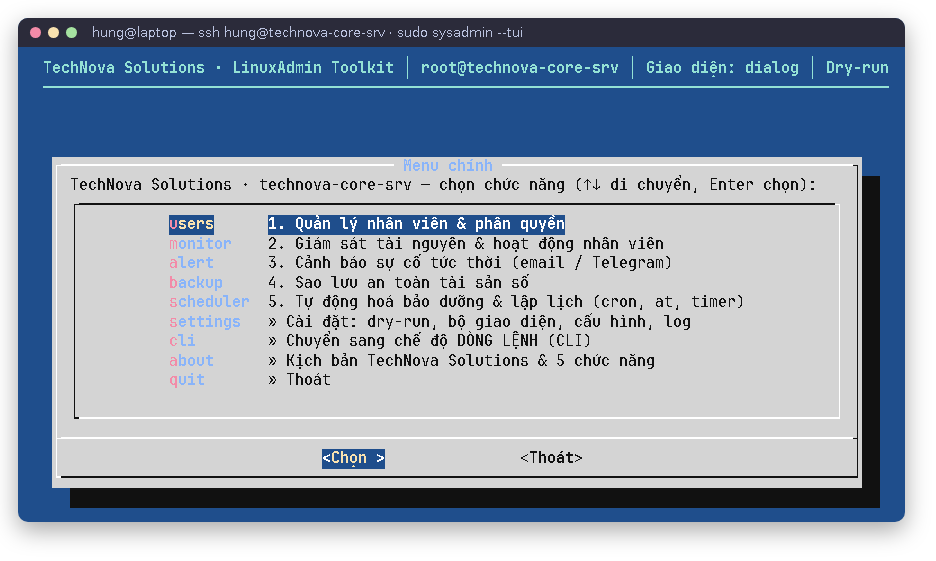
\includegraphics[width=0.86\textwidth]{tui-main.png}
\caption{Menu chính của giao diện TUI khi SSH vào technova-core-srv}\label{fig:tui}\end{figure}
\begin{figure}[H]\centering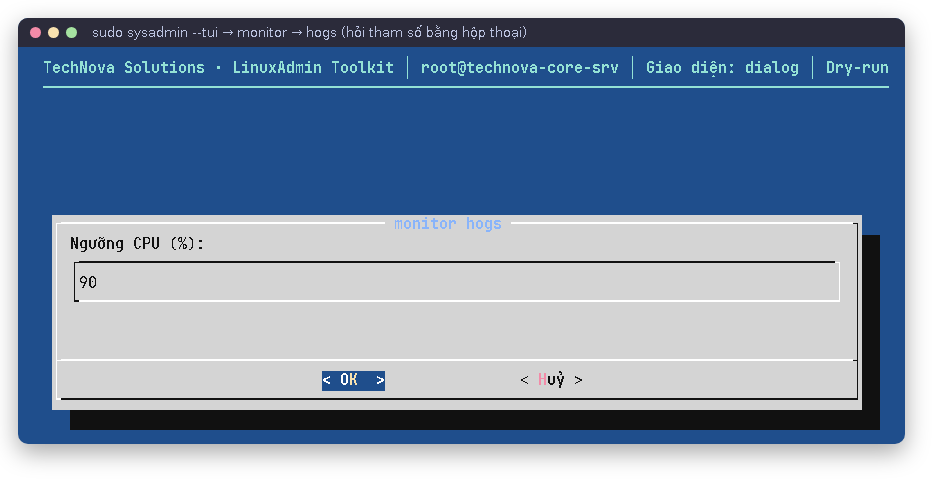
\includegraphics[width=0.86\textwidth]{tui-result.png}
\caption{Giao diện hỏi tham số bằng hộp thoại (monitor → hogs)}\label{fig:tuiparam}\end{figure}

\section{Chức năng 1 — users: quản lý nhân viên và phân quyền}
Danh sách nhân viên được khai báo trong \cmd{config/users.csv}. Mỗi dòng gồm username, họ tên, phòng ban, shell và quyền sudo. Lệnh \cmd{users create} xử lý từng nhân viên theo các bước:
\begin{enumerate}
  \item kiểm tra tên hợp lệ bằng biểu thức chính quy;
  \item bỏ qua nếu tài khoản đã tồn tại;
  \item tạo nhóm phòng ban nếu chưa có;
  \item gọi \cmd{useradd} với nhóm phụ (thêm nhóm sudo/wheel nếu được cấp quyền);
  \item đặt mật khẩu ngẫu nhiên 12 ký tự qua \cmd{chpasswd};
  \item ép đổi mật khẩu ở lần đăng nhập đầu và áp chính sách hết hạn (\cmd{chage -d 0 -M 90 -m 1 -W 7}).
\end{enumerate}
Mật khẩu tạm được lưu vào một tệp CSV có quyền \cmd{600}.

Lệnh \cmd{users setup-dirs} tạo cây thư mục dự án: \cmd{/srv/technova/\{dev,data,qa\}} với quyền \cmd{2770} và bit SGID, cùng thư mục \cmd{chung/} với quyền \cmd{1777} và sticky bit. Lệnh \cmd{users demo} tự động \textbf{thử quyền truy cập thực tế} dưới danh nghĩa từng nhân viên bằng \cmd{runuser} (Hình~\ref{fig:usersdemo}).

\begin{figure}[H]\centering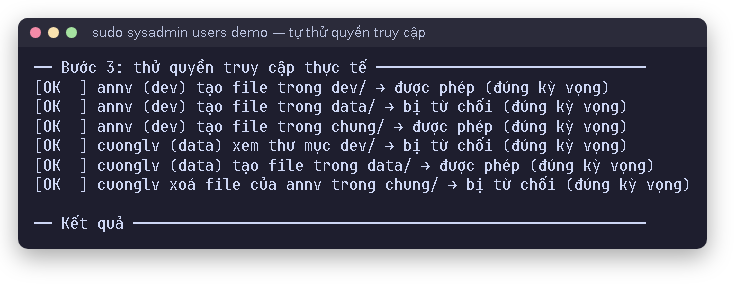
\includegraphics[width=0.92\textwidth]{users-demo.png}
\caption{Kiểm chứng phân quyền theo phòng ban}\label{fig:usersdemo}\end{figure}

Khi nhân viên nghỉ việc, lệnh \cmd{users offboard} thực hiện liền một quy trình 5 bước (Hình~\ref{fig:offboard}):
\begin{enumerate}
  \item khoá mật khẩu và đặt ngày hết hạn tài khoản (\cmd{usermod -L -e 1}), chặn cả đăng nhập bằng SSH key;
  \item ngắt mọi phiên làm việc (\cmd{loginctl terminate-user}, \cmd{pkill -KILL -u});
  \item thu hồi quyền sudo;
  \item xoá crontab cá nhân;
  \item nén thư mục home để lưu trữ.
\end{enumerate}
Lệnh \cmd{users audit} kiểm tra bảo mật trên 10 nhóm tiêu chí: tài khoản UID 0, mật khẩu rỗng hoặc không hết hạn, quyền của \cmd{/etc/shadow} và \cmd{/etc/sudoers}, quy tắc NOPASSWD, quyền thư mục home, tệp ai cũng ghi được, tệp SUID và cấu hình SSH.

\begin{figure}[H]\centering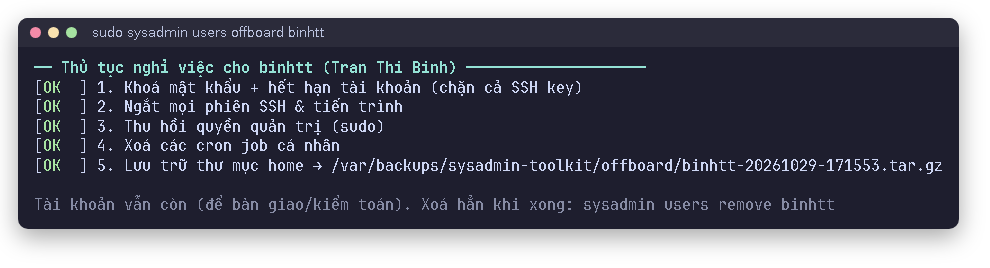
\includegraphics[width=0.86\textwidth]{offboard.png}
\caption{Quy trình nhân viên nghỉ việc (offboard)}\label{fig:offboard}\end{figure}

\section{Chức năng 2 — monitor: giám sát tài nguyên và nhân viên}
\begin{itemize}
  \item \cmd{monitor who} trả lời câu hỏi \textit{ai đang đăng nhập, từ IP nào, đang chạy lệnh gì} (dùng \cmd{w}, \cmd{last}, \cmd{lastb}).
  \item \cmd{monitor usage} cộng dồn CPU/RAM \textbf{theo từng nhân viên} bằng \cmd{awk}:
\end{itemize}
\begin{Verbatim}
ps -eo user:20=,uid=,pcpu=,pmem=,rss= | awk -v min="$UID_MIN" '
  { u=$1; p[u]++; c[u]+=$3; m[u]+=$4; r[u]+=$5; id[u]=$2 }
  END { for (u in p) printf "%.1f\t%s %d %.1f %.1f %.0f\n",
        c[u], u, p[u], c[u], m[u], r[u]/1024 }' | sort -rn
\end{Verbatim}
\begin{itemize}
  \item \cmd{monitor hogs} lọc các process vượt ngưỡng (mặc định $\ge$ 90\% CPU hoặc $\ge$ 30\% RAM) và hiển thị dòng lệnh đầy đủ, giúp nhận ra ngay ai đang treo process gì (Hình~\ref{fig:hogs}).
  \item Để xử lý, Tech Lead có thể hạ độ ưu tiên bằng \cmd{monitor renice} (mềm mỏng) hoặc dừng tiến trình bằng \cmd{monitor kill}. Lệnh kill có xác nhận và từ chối PID 1.
\end{itemize}

\begin{figure}[H]\centering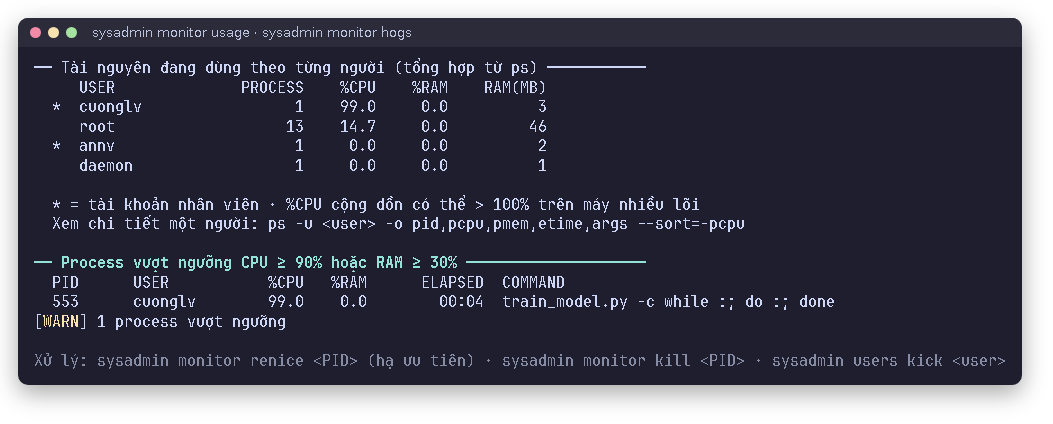
\includegraphics[width=0.95\textwidth]{monitor-hogs.png}
\caption{Phát hiện Data Analyst \texttt{cuonglv} treo \texttt{train\_model.py} chiếm 99\% CPU}\label{fig:hogs}\end{figure}

Ngoài ra, module còn có:
\begin{itemize}
  \item \cmd{troubleshoot}: quy trình chẩn đoán 10 bước (tải, CPU, iowait, RAM/swap, OOM, đĩa/inode, dịch vụ lỗi, mạng/DNS, log lỗi, NTP/zombie), kèm gợi ý xử lý;
  \item \cmd{report}: xuất báo cáo HTML có biểu đồ CPU/RAM theo thời gian;
  \item \cmd{watch}: bảng theo dõi thời gian thực.
\end{itemize}

\section{Chức năng 3 — alert: cảnh báo sự cố tức thời}
\cmd{alert check} được cron gọi mỗi 5 phút và thực hiện tuần tự:
\begin{enumerate}
  \item đo CPU (lấy mẫu \cmd{/proc/stat}), RAM, ổ đĩa, rồi ghi vào \cmd{metrics.csv};
  \item phát hiện process ngốn tài nguyên, kèm tên nhân viên đang chạy;
  \item phát hiện dịch vụ systemd bị lỗi;
  \item đếm số lần đăng nhập SSH thất bại trong 10 phút (dấu hiệu bị dò mật khẩu);
  \item nếu có sự cố, gửi cảnh báo qua \textbf{email} (msmtp/mail) và \textbf{Telegram} (gọi Bot API bằng \cmd{curl}).
\end{enumerate}
Có \textbf{thời gian chờ (cooldown) 30 phút} để không gửi trùng lặp lúc nửa đêm. Khi hết sự cố, toolkit gửi tin \textbf{``đã ổn định''}. Tiêu đề email tiếng Việt được mã hoá theo RFC 2047 (\cmd{=?UTF-8?B?...?=}).

\begin{figure}[H]\centering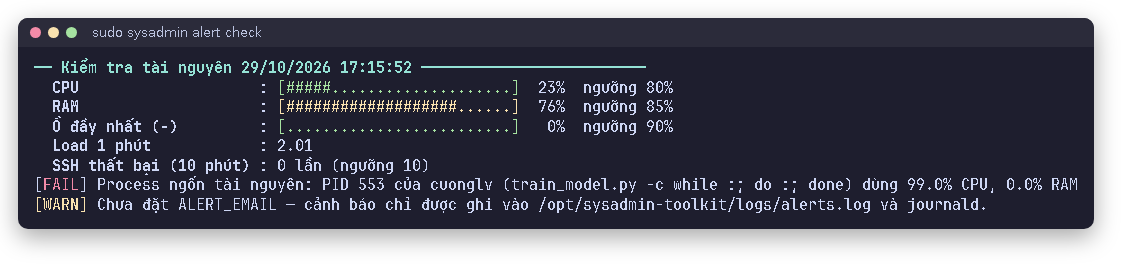
\includegraphics[width=0.95\textwidth]{alert-check.png}
\caption{alert check phát hiện process ngốn tài nguyên}\end{figure}

\section{Chức năng 4 — backup: sao lưu tài sản số}
Dữ liệu được sao lưu mặc định gồm \cmd{/srv/technova} (dự án), \cmd{/home} (nhân viên) và \cmd{/etc} (cấu hình). Một lần sao lưu đi qua các bước sau:
\begin{enumerate}
  \item khoá \cmd{flock} để chống chạy trùng;
  \item nén bằng \cmd{tar -czp} (bỏ qua tệp không đọc được thay vì làm hỏng cả bản sao);
  \item kiểm tra tệp nén (\cmd{gzip -t});
  \item tạo checksum SHA-256;
  \item xoay vòng, giữ 7 bản mới nhất;
  \item tuỳ chọn \cmd{rsync} bản sao ra máy khác;
  \item ghi lịch sử, và gửi cảnh báo nếu thất bại.
\end{enumerate}
\begin{Verbatim}
exec 9>"$dest/.backup.lock"
flock -n 9 || die "Đang có một tiến trình sao lưu khác chạy."
tar -czpf "$file" --ignore-failed-read "${excl[@]}" -C / "${rel[@]}"
gzip -t "$file" && (cd "$dest" && sha256sum "$name" > "$name.sha256")
\end{Verbatim}
\begin{figure}[H]\centering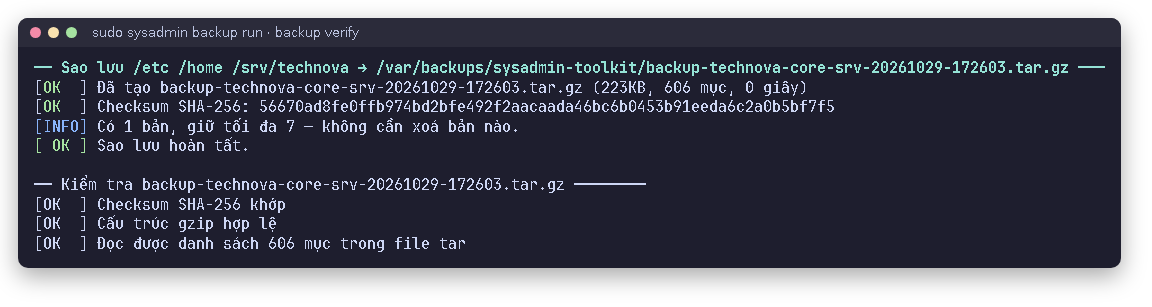
\includegraphics[width=0.95\textwidth]{backup.png}
\caption{Sao lưu và kiểm tra toàn vẹn bản sao}\end{figure}

\section{Chức năng 5 — scheduler: tự động hoá bảo dưỡng}
\cmd{scheduler install} ghi một \textbf{khối lịch riêng} vào crontab của root, nằm giữa hai dòng đánh dấu \cmd{>>> sysadmin-toolkit >>>}. Nhờ vậy, cài lại hay gỡ bỏ đều không ảnh hưởng các job khác của hệ thống.

\begin{table}[H]\centering\small\caption{Lịch tự động mặc định}
\begin{tabularx}{\textwidth}{>{\raggedright\arraybackslash}p{3.4cm}>{\raggedright\arraybackslash}p{3.0cm}L}\toprule
\textbf{Biểu thức cron} & \textbf{Thời điểm} & \textbf{Tác vụ}\\\midrule
\cmd{0 2 * * *} & 02:00 hằng ngày & \cmd{backup run}\\
\cmd{30 3 * * *} & 03:30 hằng ngày & \cmd{scheduler maintenance}: dọn /tmp, log journald cũ, cache gói, core dump, xoay vòng backup\\
\cmd{*/5 * * * *} & mỗi 5 phút & \cmd{alert check}\\
\cmd{0 7 * * 1} & 07:00 thứ Hai & \cmd{monitor report}\\\bottomrule
\end{tabularx}\end{table}
\begin{figure}[H]\centering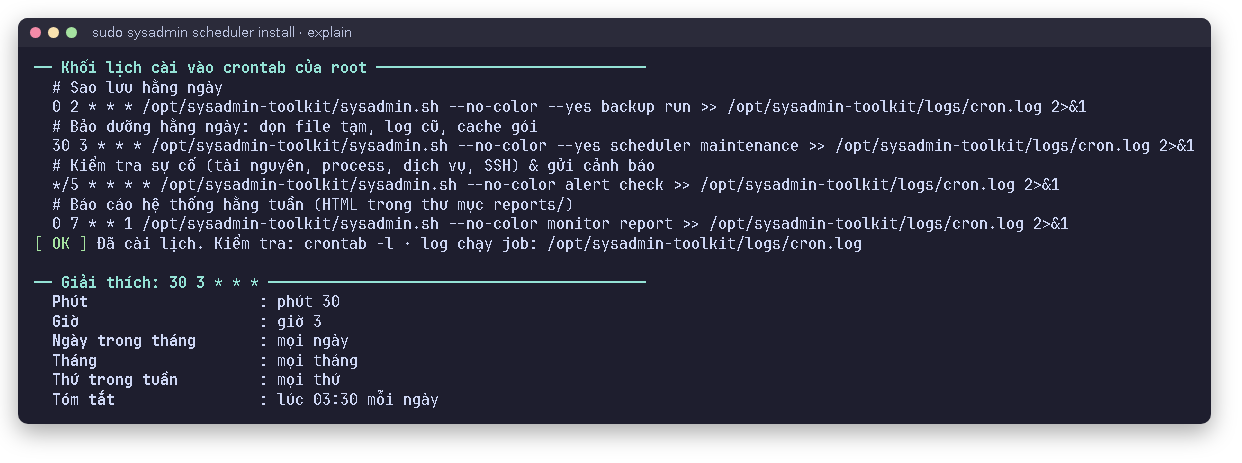
\includegraphics[width=0.95\textwidth]{scheduler.png}
\caption{Cài lịch tự động và giải thích biểu thức cron bằng tiếng Việt}\end{figure}

Toolkit cũng có thể dùng systemd timer thay cho cron (\cmd{scheduler timers-install}), và hỗ trợ hẹn giờ chạy một lần bằng \cmd{at}.

\section{Đóng gói và triển khai}
\begin{itemize}
  \item \textbf{Cài trên máy thật:} \cmd{sudo ./install.sh --deps} chép toolkit vào \cmd{/opt/sysadmin-toolkit} (chủ sở hữu root), tạo lệnh \cmd{sysadmin}, cài các gói phụ thuộc và bật tự hoàn thành lệnh bằng phím Tab.
  \item \textbf{Docker:} \cmd{docker compose up -d} dựng sẵn máy chủ \cmd{technova-core-srv} (Ubuntu 24.04, cron, at, SSH server). Tech Lead SSH vào cổng 2222 như với máy thật; bản sao lưu, cấu hình, báo cáo và log được giữ trong volume.
  \item \textbf{Gói nén:} \cmd{./package.sh} tạo tệp \cmd{.tar.gz} kèm checksum để mang sang máy Linux khác.
\end{itemize}

% ================================================================ CHƯƠNG 5 ===
\chapter{Kiểm thử và đánh giá}

\section{Môi trường kiểm thử}
\begin{itemize}
  \item \textbf{Ubuntu 24.04} chạy trong container Docker, hostname \cmd{technova-core-srv}, quyền root, có \cmd{CAP\_SYS\_NICE}.
  \item \textbf{Kali Linux Rolling} (kernel 7.1, bash 5.3), tài khoản thường: chạy các chức năng chỉ đọc và chế độ dry-run.
  \item Kiểm tra tĩnh bằng \textbf{shellcheck}.
\end{itemize}

\section{Kịch bản kiểm thử tự động}
Script \cmd{tests/demo-test.sh} mô phỏng trọn ``một ngày của anh Hưng'' theo thứ tự: nhân viên mới vào làm → một nhân viên treo process → cảnh báo → sao lưu → tự động hoá → nhân viên nghỉ việc → dọn dẹp. Mỗi bước được kiểm chứng bằng điều kiện cụ thể trên hệ thống, ví dụ: thành viên nhóm, quyền thư mục, tiến trình còn sống hay không, nội dung crontab, nội dung tệp khôi phục.

\begin{table}[H]\centering\small
\caption{Kết quả kiểm thử tự động}
\begin{tabularx}{\textwidth}{>{\raggedright\arraybackslash}p{4.3cm}Lcc}\toprule
\textbf{Nhóm} & \textbf{Nội dung kiểm chứng} & \textbf{Số test} & \textbf{Kết quả}\\\midrule
0. Nền tảng & Phiên bản, help sinh tự động, từ chối tham số sai, dry-run không thay đổi hệ thống & 5 & 5/5\\
1. users & Tạo 7 nhân viên, phòng ban, sudo, ép đổi mật khẩu, tệp mật khẩu 600, idempotent, quyền 2770/1777, SGID, sticky, lock/unlock, audit & 18 & 18/18\\
2. monitor & Mô phỏng process treo, usage, hogs, top, who/overview/troubleshoot, renice & 6 & 6/6\\
3. alert & Phát hiện sự cố, ghi log, cooldown, kill, tin ``đã ổn định'', metrics.csv, đổi ngưỡng & 7 & 7/7\\
4. backup & Tạo bản sao, SHA-256 khớp, chứa dữ liệu dự án, verify, khôi phục đúng nội dung, xoay vòng & 6 & 6/6\\
5. scheduler & Khối cron đủ 4 job, job tuỳ chỉnh (thoát \%), explain, từ chối cron sai, bảo dưỡng xoá tệp cũ, gỡ lịch & 7 & 7/7\\
1'. Nghỉ việc & kick, offboard (khoá + lưu trữ home), từ chối offboard root & 4 & 4/4\\
Dọn dẹp & Xoá nhân viên, thư mục, nhóm demo & 2 & 2/2\\\midrule
\textbf{Tổng} & & \textbf{55} & \textbf{55/55}\\\bottomrule
\end{tabularx}
\end{table}

Chạy lại bộ kiểm thử bằng lệnh:
\begin{Verbatim}
docker run --rm --cap-add SYS_NICE -v "$PWD/tests:/tests:ro" \
       technova/sysadmin-toolkit:1.0 bash /tests/demo-test.sh --yes
\end{Verbatim}

\section{Đánh giá lợi ích của tự động hoá}
\begin{table}[H]\centering\small
\caption{So sánh thao tác thủ công và dùng toolkit (ước tính của nhóm)}
\begin{tabularx}{\textwidth}{>{\raggedright\arraybackslash}p{4.4cm}>{\raggedright\arraybackslash}p{4.6cm}L}\toprule
\textbf{Công việc} & \textbf{Làm tay} & \textbf{Với toolkit}\\\midrule
Tạo 7 nhân viên + phòng ban + thư mục & $\approx$ 50 lệnh, 20–30 phút, dễ sai quyền & 2 lệnh, $<$ 10 giây, có kiểm chứng\\
Tìm ai đang treo process & \cmd{ps}/\cmd{top}, tự đối chiếu user & \cmd{monitor hogs}: một lệnh\\
Phát hiện sự cố lúc 2 giờ sáng & Chỉ biết khi nhân viên phản ánh & Cảnh báo trong $\le$ 5 phút\\
Sao lưu hằng ngày & Dễ quên, không kiểm tra bản sao & Tự động, có checksum và xoay vòng\\
Nhân viên nghỉ việc & Dễ sót bước (sudo, crontab, phiên còn mở) & \cmd{users offboard}: 5 bước một lần\\\bottomrule
\end{tabularx}
\end{table}

\section{Hạn chế}
\begin{itemize}
  \item Chỉ quản lý một máy chủ; chưa có cơ chế quản lý tập trung nhiều máy.
  \item Bản Docker không có systemd, nên chức năng systemd timer và log journald bị hạn chế (vẫn dùng cron được).
  \item Gửi email phụ thuộc vào cấu hình SMTP bên ngoài (Gmail App Password); nhóm chưa kiểm thử gửi thư thật.
  \item Giao diện whiptail cần nhấn Tab để đóng hộp kết quả; dùng \cmd{dialog} sẽ thuận tiện hơn.
\end{itemize}

% ================================================================ CHƯƠNG 6 ===
\chapter{Kết luận và hướng phát triển}
\section{Kết luận}
Đồ án đã xây dựng thành công \textbf{LinuxAdmin Toolkit}. Bộ công cụ chứng minh rằng Bash scripting đủ sức tự động hoá toàn bộ công việc quản trị hằng ngày của một máy chủ doanh nghiệp, cụ thể:
\begin{itemize}
  \item quản lý vòng đời nhân viên, từ tiếp nhận đến nghỉ việc;
  \item phân quyền theo phòng ban;
  \item giám sát và xử lý tiến trình gây sự cố;
  \item cảnh báo tức thời;
  \item sao lưu an toàn;
  \item bảo dưỡng định kỳ.
\end{itemize}
Thiết kế ``giao diện là lớp vỏ của CLI'' giúp toolkit vừa thân thiện qua SSH, vừa dễ dùng trong script và cron. Bộ kiểm thử tự động 55 bước xác nhận các chức năng hoạt động đúng.

\section{Hướng phát triển}
\begin{itemize}
  \item Quản lý nhiều máy chủ qua SSH hoặc chuyển sang Ansible.
  \item Dashboard web đọc dữ liệu \cmd{metrics.csv} và báo cáo.
  \item Tích hợp xác thực hai lớp và theo dõi lệnh sudo của nhân viên (\cmd{auditd}).
  \item Đẩy bản sao lưu lên dịch vụ lưu trữ đám mây và mã hoá bản sao bằng GPG.
\end{itemize}

% ================================================================ PHỤ LỤC ===
\appendix
\renewcommand{\chapname}{PHỤ LỤC}
\chapter{Hướng dẫn cài đặt nhanh}
\begin{Verbatim}
# Cách A — Docker (máy chủ giả lập technova-core-srv)
git clone https://github.com/duylmaoxd/technova-sysadmin-toolkit.git
cd technova-sysadmin-toolkit && docker compose up -d --build
ssh -p 2222 hung@localhost        # rồi: sudo sysadmin --tui

# Cách B — cài trực tiếp trên Ubuntu Server
sudo ./install.sh --deps
sudo sysadmin scheduler install
\end{Verbatim}
Mã nguồn: \url{\RepoURL}. Hướng dẫn chi tiết: tệp \cmd{HUONG-DAN-SU-DUNG.md}.

\chapter{Danh sách lệnh}
\begin{longtable}{>{\raggedright\arraybackslash}p{2.4cm}>{\raggedright\arraybackslash}p{12.2cm}}
\toprule\textbf{Chức năng} & \textbf{Action}\\\midrule\endhead
users & list, create, delete, add, remove, lock, unlock, passwd, sudo, policy, set-policy, audit, perm, shared-dir, setup-dirs, kick, offboard, demo, demo-clean\\
monitor & who, usage, top, hogs, renice, kill, overview, memory, disk, logs, auth, troubleshoot, report, watch, history\\
alert & check, status, test, setup-mail, setup-telegram, set-threshold, stress, history\\
backup & run, list, verify, restore, rotate, history\\
scheduler & list, install, maintenance, remove, add, explain, at, at-list, at-remove, log, timers-install, timers-remove\\\bottomrule
\end{longtable}
Tuỳ chọn chung: \cmd{--tui}, \cmd{--cli}, \cmd{--dry-run}, \cmd{--yes}, \cmd{--ascii}, \cmd{--no-color}, \cmd{--config}. Xem chi tiết: \cmd{sysadmin help <chức năng>}.

\end{document}
